\documentclass[12pt,a4paper]{article}
\usepackage[utf8]{inputenc}
\usepackage{graphicx}
\usepackage{amsmath, amsthm, amssymb}
\usepackage{changepage}
\usepackage[a4paper,includeheadfoot,margin=2.54cm]{geometry}
\usepackage{caption}
\newtheorem{theorem}{Theorem}

\begin{document}

\section{The Koch Snowflake}

The \emph{Koch snowflake},
one of the first fractals, is based on work by the Swedish mathe-
matician Helge von Koch~\cite{koch}.
\begin{figure}[h]
	\centering
	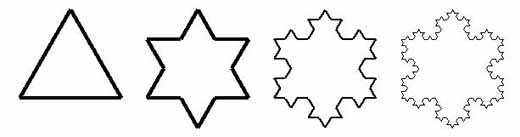
\includegraphics[width=10cm]{snowflake.jpg}
	\caption{The Koch snowflake after 0, 1, 2, and 3 iterations.}
	\label{koch}
\end{figure}
It is what we get if we start with an equilateral triangle    and repeat the following an infinite number of times:
\begin{quote}
\textit{Divide all line segments into three segments of equal length. Then draw, for each middle line segment, an equilateral triangle that has the middle segment as its base and points outward. Finally, remove all middle segments.}
\end{quote}
\begin{adjustwidth}{0cm}{-2cm}
Figure~\ref{koch} shows the first iterations in the construction.\hfill(Original)
\end{adjustwidth}
\section{Two properties}
\begin{theorem}
  The Koch snowflake has infinite length. 
\end{theorem}
\begin{proof}
  Let
  $\Delta$
  denote a triangle, with side length $s$, on which we base the construction of a snowflake.
  Let
  $N_i$ 
  denote the number of line segments, 
  and
  $L_i$ 
  the length of the segments, in iteration $i$ of the construction.
  Then
  \begin{displaymath}
    N_n =
    \begin{cases}
      3, & \text{if $n=0$ (i.e. before any iterations), and} \\4N_{n-1}, & \text{otherwise.}
    \end{cases}
  \end{displaymath}
  This solves to
  \begin{equation}
    \label{eq:1}
    N_n = 3 \cdot 4^n,
  \end{equation}
   while  
  \begin{equation}
    \label{eq:5}
    L_n = \frac{L_{n-1}}{3} = \frac{L_{n-2}}{3^2} = \frac{L_{n-3}}{3^3} = \ldots = \frac{L_0}{3^n} = \frac{s}{3^n}
  \end{equation}
  From Eqs.~\ref{eq:1}  and~\ref{eq:5}, the total length
  \begin{displaymath}
    N_nL_n = 3 \cdot 4^n\frac{s}{3^n} = 3s\frac{4^n}{3^n} = 3s\left(\frac{4}{3}\right)^n.
  \end{displaymath}
  Since 4$/$3 $>$ 1, it follows that $N_nL_n$ tends to infinity as $n \to \infty$, which means the Koch snowflake indeed has infinite length.
\end{proof}

\begin{theorem}
	The Koch snowflake has finite area.
\end{theorem}
\begin{proof}  
  In an iteration, a single triangle is added on each line segment of the previous iteration. So, in iteration $n$, the number of new triangles $T_n = N_{n-1}$, which, by Eq.~\ref{eq:1}, can be simplified to 
	\begin{equation}
		\label{eq:2}
		T_n = \frac{3}{4} \cdot 4^n.
	\end{equation}
	The area $a_n$ of each such triangle, with the exception of the area
	\begin{displaymath}
		a_n = \frac{\sqrt{3}}{4}s^2
	\end{displaymath}
	of $\Delta$, the initial equilateral triangle, is one ninth of the area of a triangle added in iteration $n - 1$, or 
	\begin{equation}
    	\label{eq:3}
    	a_n = \frac{a_{n-1}}{9} = \frac{a_{n-2}}{9^2} =  \ldots = \frac{a_1}{9^{n-1}} = \frac{a_0}{9^n}..
    \end{equation}
    This means that in iteration $n$, by Eqs.~\ref{eq:2} and \ref{eq:3}, the area of all added triangles
    \begin{equation}
    	b_n = T_na_n = \left(\frac{3}{4} \cdot 4^n \right) \left(\frac{a_0}{9^n}\right)  = \frac{3a_0}{4} \left(\frac{4}{9}\right)^n.
    \end{equation}
    All in all, after iteration $n$, the total area
    \begin{align*}
    	A_n &= a_0 + \sum_{k=1}^nb_k \\
    	&= a_0\left(1 + \frac{3}{4}\sum_{k=1}^n\left(\frac{4}{9}\right)^k\right) \\
    	&= a_0\left(1 + \frac{1}{3}\sum_{k=0}^{n-1}\left(\frac{4}{9}\right)^k\right) \\
    	&= a_0\left(1 + \frac{3}{5}\left(1 - \left(\frac{4}{9}\right)^n\right)\right) \\
    	&= \frac{a_0}{5}\left(8 - 3\left(\frac{4}{9}\right)^n\right).
    \end{align*}
    Now, since the denominator is larger than the numerator,
    \begin{displaymath}
    	\lim_{n\to\infty} 3\left(\frac{4}{9}\right)^n = 0,
    \end{displaymath}
    it follows that $\lim_{\to \infty} A_n$. This shows that the Koch snowflake indeed has finite area.  
\end{proof}


\begin{thebibliography}{99}
  \bibitem{koch} Helge. \emph{Sur une courbe continue sans
      tangente, obtenue par une construction géométrique
      élémentaire.}, Arkiv,
    Kungliga Vetenskapsakademien. \textbf{1}, 681-702,.
\end{thebibliography}
\end{document}